%!TEX root = mb.tex
\begin{figure}[t]
  \centering
  \begin{tabular}{cc}
  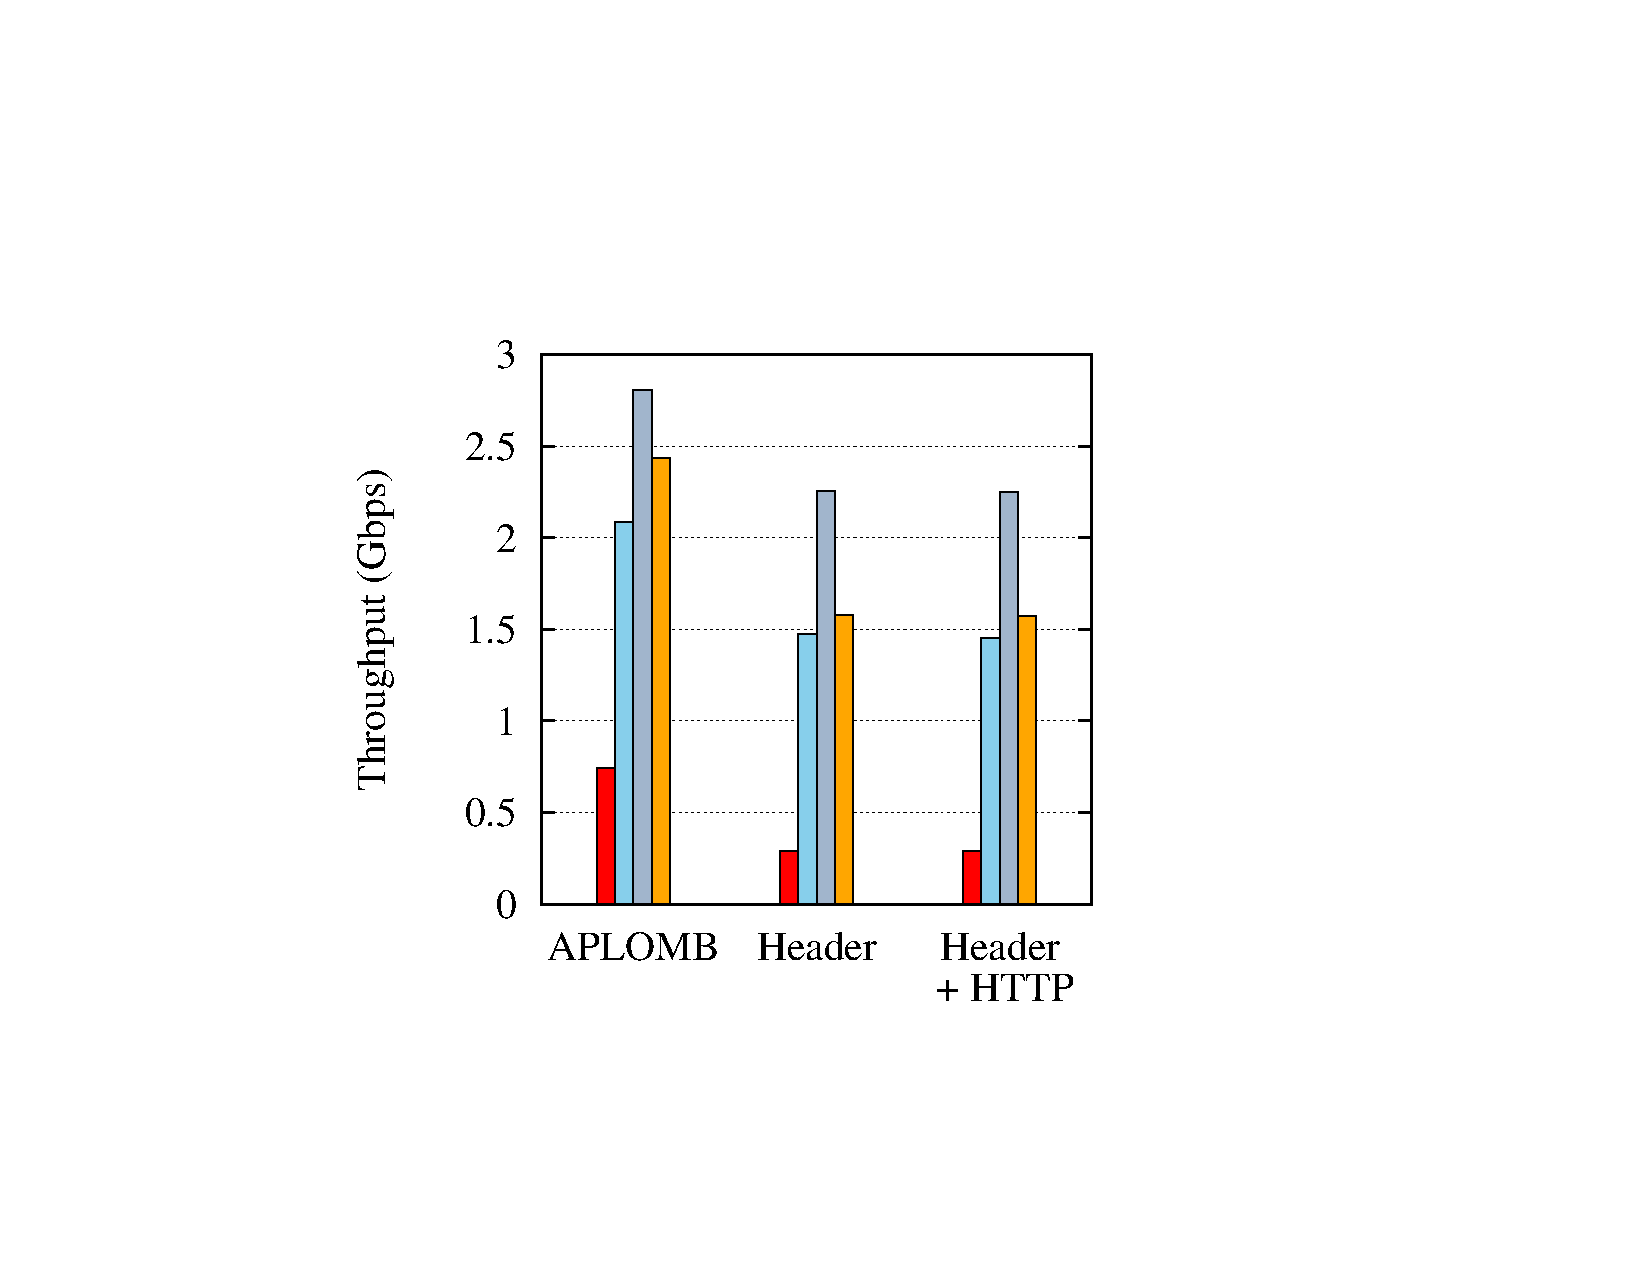
\includegraphics[height=1in]{fig/gatewayxput}&
  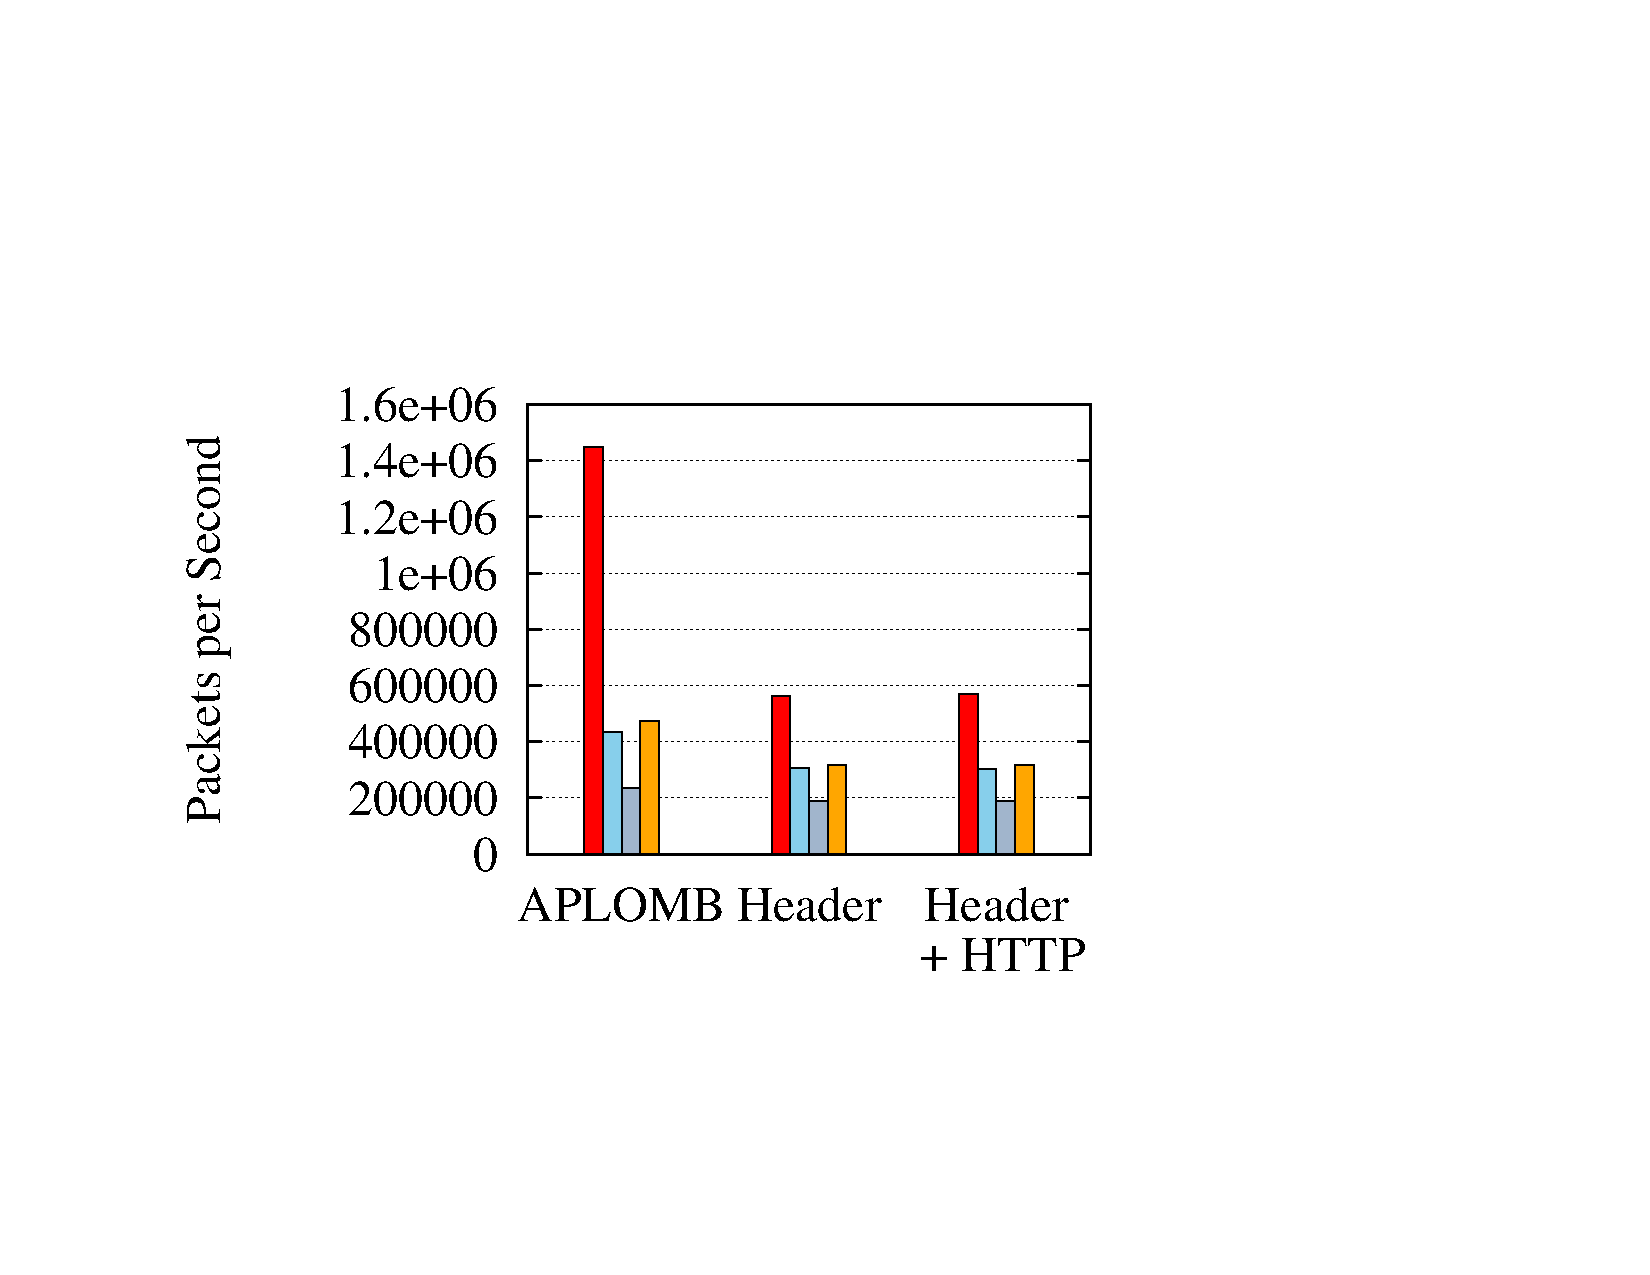
\includegraphics[height=1in]{fig/gateway_pps}\\
  \end{tabular}
  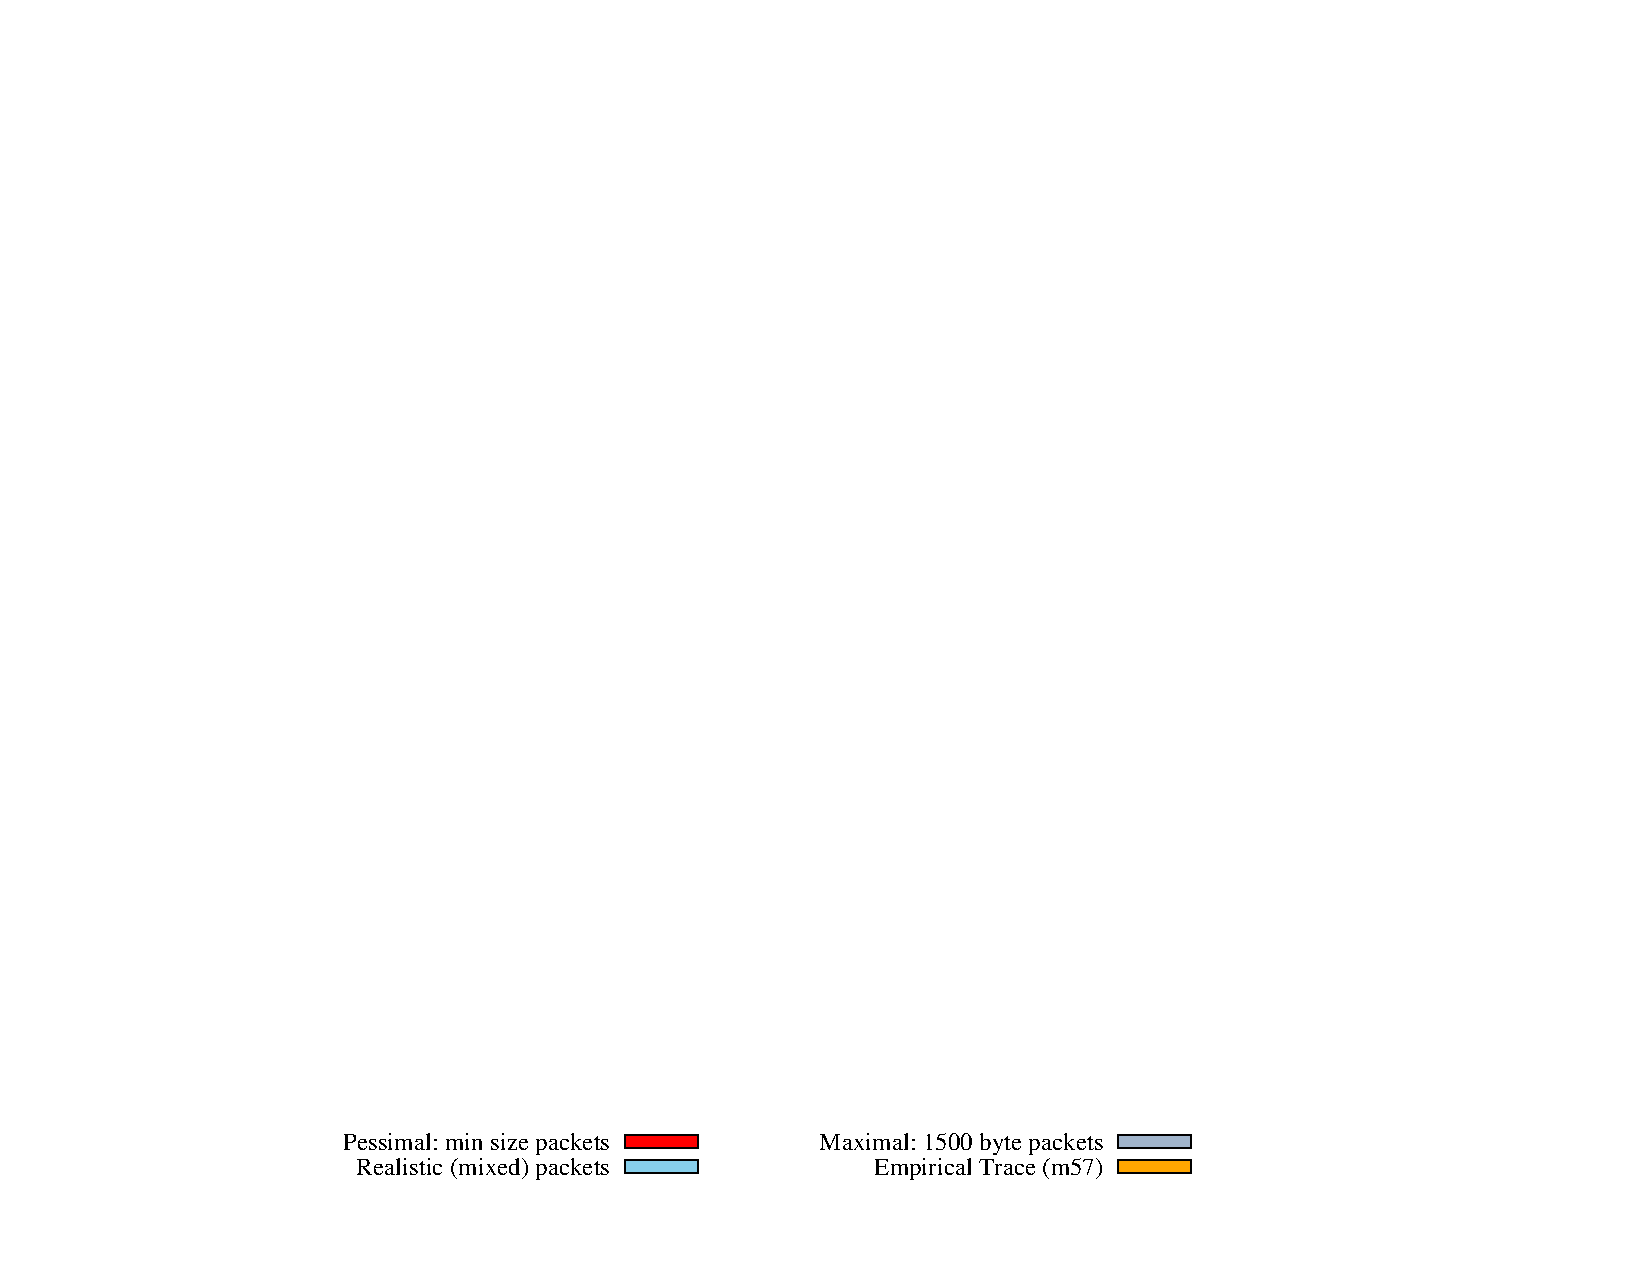
\includegraphics[width=2.75in]{fig/key}
  \caption[]{\label{fig:gwxput} Throughput/Packets per Second on a single core at the stateless gateway.}
\end{figure}

\begin{figure}[t]
  \centering
  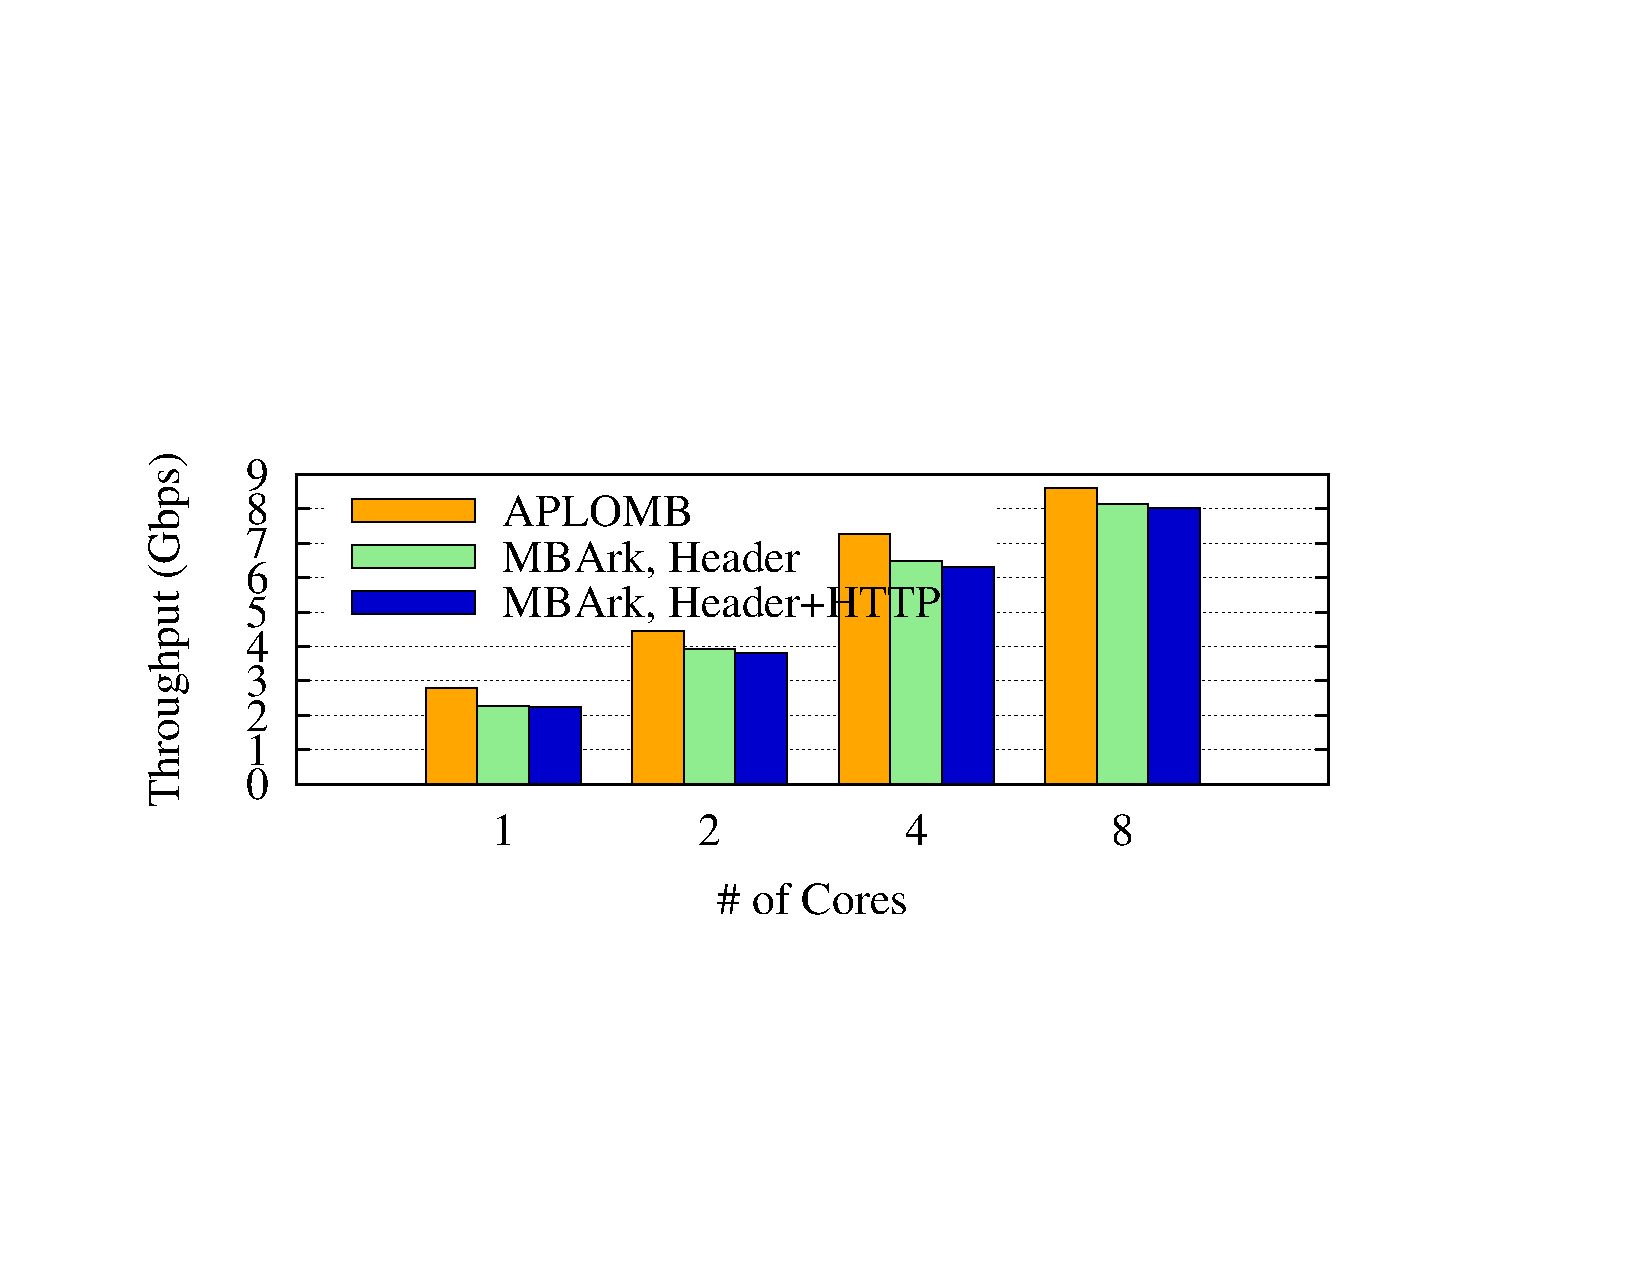
\includegraphics[width=3in]{fig/gateway_scale}
  \caption[]{\label{fig:gwscale} Gateway throughput with increasing parallelism.}
\end{figure}
 
\section{Evaluation} \label{sec:eval}

As we showed in \S\ref{sec:mbs}, \sys supports all middlebox applications in typical outsourcing environments~\cite{aplomb,nfv} -- including header-only middleboxes as well as bytestream-aware middleboxes . 
Hence, from a functionality perspective, \sys answers our original question, ``Is it possible to enable a third party to perform traffic processing for an enterprise, {\em without seeing the enterprise's traffic}?''  strongly in the affirmative.

We now investigate whether \sys is practical from a performance perspective, looking at the overheads due to encryption (over the header or the payload) and redirection. 
%\sys has very low hardware overheads at the enterprise: our eight-core server could easily saturate a 10Gbps link with encrypted traffic to and from the cloud; we evaluate the gateway throughput in \S\ref{sec:gateway}.
%Because most middleboxes are unchanged in the dataplane, throughput overheads at the cloud due to \sys are negligible, typically under 1\%, as we show in \S\ref{sec:homiddleboxes}.  

%We ran our experiments using the implementation described in \ref{sec:impl}. 
%Our prototype gateway runs with four 2.6GHz Xeon E5-2650 cores and 128 GB RAM; the network hardware is a single 10GbE Intel 82599 compatible network card.
We built our gateway using Click~\cite{click} over DPDK~\cite{dpdk} on an off-the-shelf 16-core server with 2.6GHz Xeon E5-2650 cores and 128GB RAM; the network hardware is a single 10GbE Intel 82599 compatible network card. 
We deployed our prototype gateway in our research lab and redirected traffic from a 3-server testbed through the gateway; these three client servers had the same hardware specifications as the server we used as our gateway.
We deployed our middleboxes on Amazon EC2.
For most experiments, we use a synthetic workload generated by the Pktgen~\cite{pktgen}; for experiments where an empirical trace is specified we use the m57 patents trace~\cite{m57} and the ICTF 2010 trace~\cite{ictf}.

%In what follows, we evaluate our performance at the enterprise, including gateway throughput, end-to-end page load times, and bandwidth costs (\S\ref{sec:enterprise}). We then evaluate performance at the cloud, evaluating each middlebox we implemented one by one (\S\ref{sec:evalcloud}).

\subsection{Enterprise Performance}
\label{sec:enterprise}
We first evaluate \sys's overheads at the enterprise. %including the gateway, end-to-end performance, and bandwidth costs from deploying \sys.

\subsubsection{Gateway}

 
\noindent{\it How many servers does a typical enterprise require to outsource traffic to the cloud?}
Figure~\ref{fig:gwxput} shows the gateway throughput when encrypting traffic to send to the cloud, first with normal redirection (as used in APLOMB~\cite{aplomb}), then with \sys's L3/L4-header encryption, and finally with L3/L4-header encryption as well as HTTP/proxy encryption. 
For empirical traffic traces with payload encryption (DPI) disabled, \sys averages 1.5Gbps per core; for full-sized packets it achieves over 2Gbps.
In scalability experiments (shown in Fig.~\ref{fig:gwscale} Our 8-core server could could forward at up to 8Gbps while encrypting headers and payloads with a combination of AES, KeywordMatch, and RangeMatch schemes.

With DPI enabled (not shown), throughput dropped to 240Mbps per core, suggesting that an enterprise would need a small cluster to reach higher bandwidth for these kinds of devices.
While DPI introduces a reduction to about one-sixth relative to other encryption schemes, there is little difference between the HTTP overhead and the L3/L4 overhead, as the HTTP encryption only occurs on HTTP requests -- a small fraction of packets. 
%Overall, \sys encryption for the stateless gateway reduces by about 60\% relative to baseline APLOMB encryption in the worst case (the min-sized workload; the reduction for the empirical (m57) workload is 38\%.  

\begin{figure}[t]
  \centering
  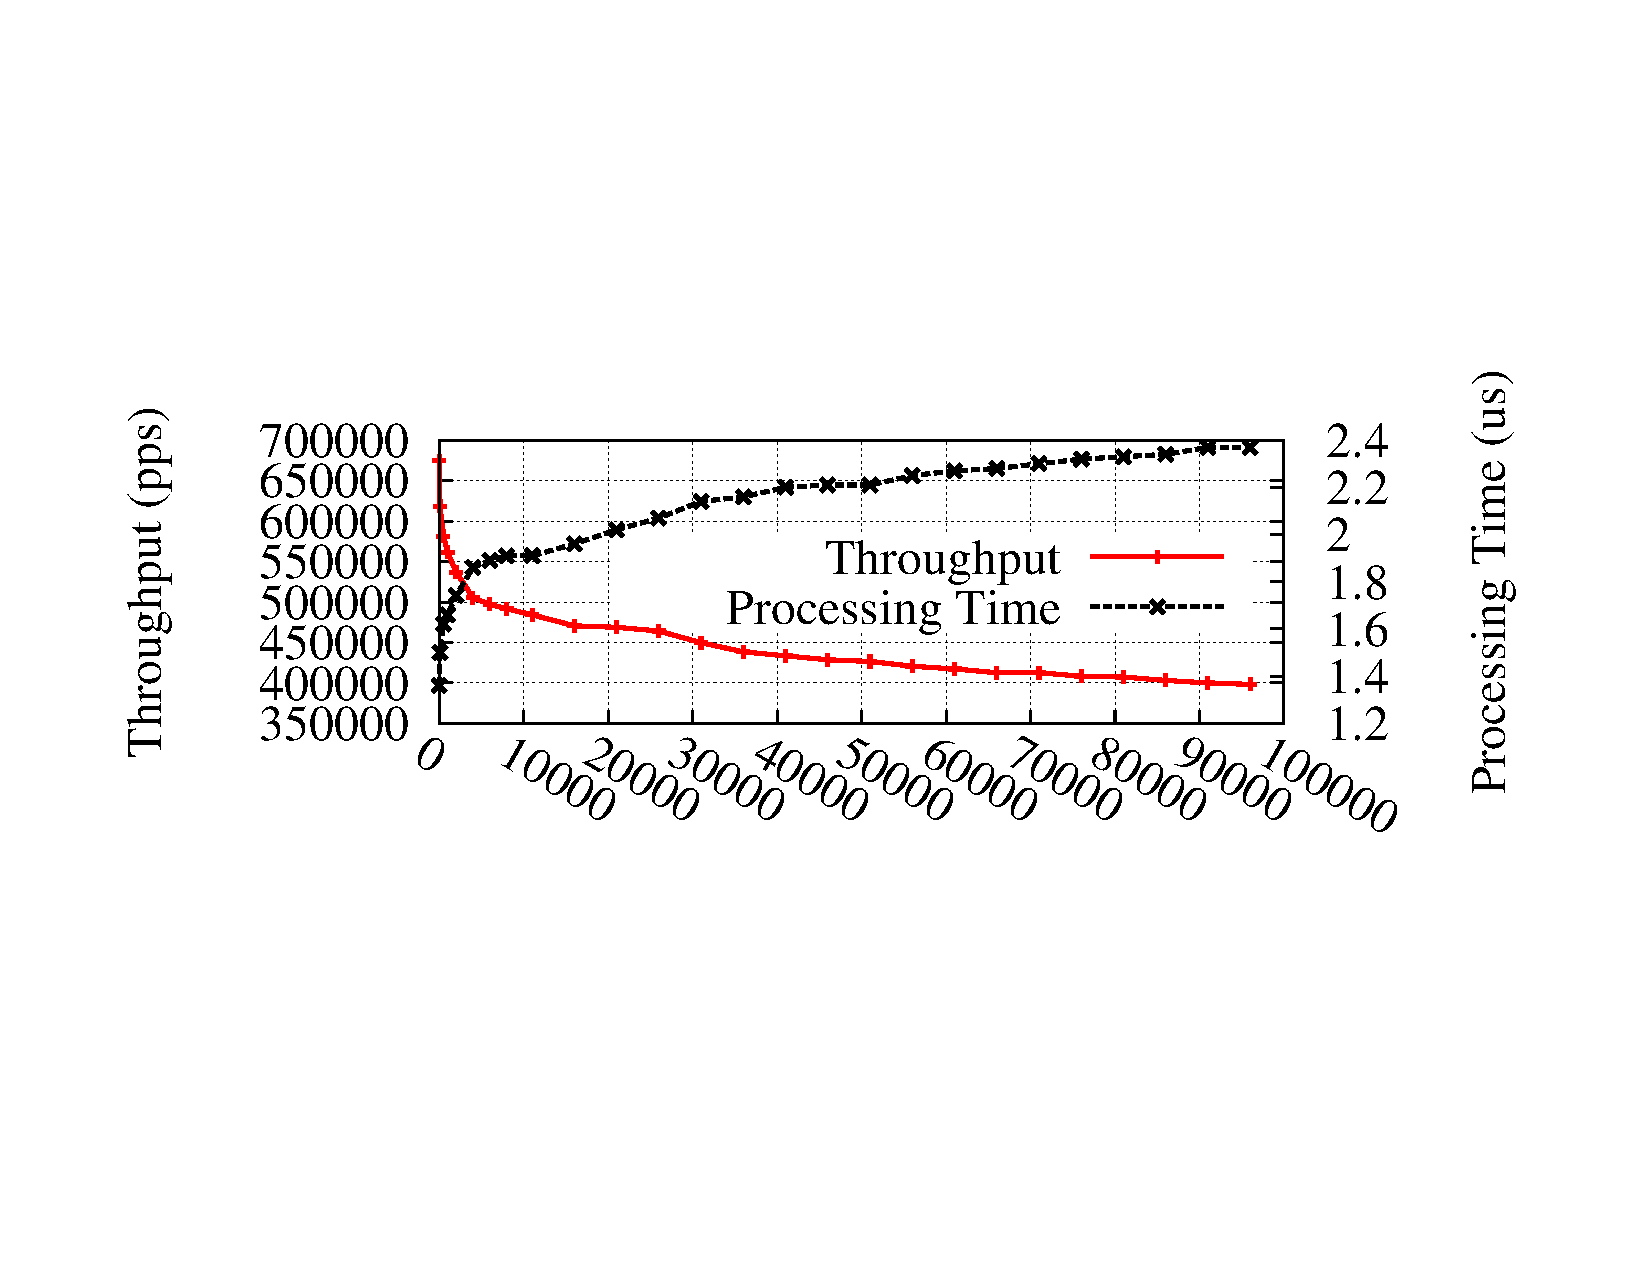
\includegraphics[width=3in]{fig/xputrange}
  \caption[]{\label{fig:xputrange} Throughput as number of rules for range encrypt increases.}
\end{figure}

\noindent{\it How do throughput and latency at the gateway scale with the number of rules for range encryption?} 
In \S\ref{sec:range}, we discussed how our range encryption scheme stores encrypted values in a tree; every packet encryption requires a traversal of this tree.
Hence, as the size of the tree goes larger, we can expect to require more time to process each packet and throughput to decrease.
We measure this effect in Figure~\ref{fig:xputrange}. 
On the $y_1$ axis, we show the aggregate per packet throughput at the gateway as the number of rules from 0 to 100k. The penalty here is logarithmic, which is the expected performance of tree data structures. From 0-10k rules, throughput drops from 670Kpps to 480Kpps; after this point the performance penalty of additional rules tapers off. Adding an additional 90k rules drops throughput to 400Kpps.
On the $y_2$ axis, we measure the processing time per packet, \ie{}, the amount of time for the gateway to encrypt the packet; the processing time follows the same logarithmic trend.

\noindent{\it Is range encryption faster than existing order preserving algorithms?}
Our range encryption is the only encryption scheme that has low enough latency for packet processing while preserving the ordering information needed for firewall rules. 
Existing order-preserving approaches require multiple round trip times -- and hence many milliseconds -- for each encryption operation.
RangeMatch encrypts each value in microseconds.
We compare against BCLO~\cite{boldyreva:ope} and mOPE~\cite{popa:mope} below:

\begin{table}[h]
\centering
\small
\begin{tabular}{c|c|c|c}
{\bf Operation}&{\bf BCLO~\cite{boldyreva:ope}}&{\bf mOPE~\cite{popa:mope}}&{\bf \sys}\\
\hline
\hline
Encrypt, 10K rules&9333$\mu$s&6640$\mu$s&1.95$\mu$s\\
\hline
Encrypt, 100K rules&9333$\mu$s&8300$\mu$s&3$\mu$s\\
\hline
Decrypt&169$\mu$s&0.128$\mu$s&0.128$\mu$s\\
\hline
\end{tabular}
\end{table}

\noindent{\it What is the memory overhead of the stateful range map encryption scheme?}
Storing 10k rules in memory requires 1.6MB, and storing 100k rules in memory requires 28.5MB -- using unoptimized C++ objects.
This state overhead is negligible on any modern server.




\subsubsection{Client Performance}

\begin{figure}
  \hspace{-15pt}
%  \begin{tabular}{cccc}
%  
\includegraphics[height=1in]{fig/cdflabel}
%  &\hspace{-10pt}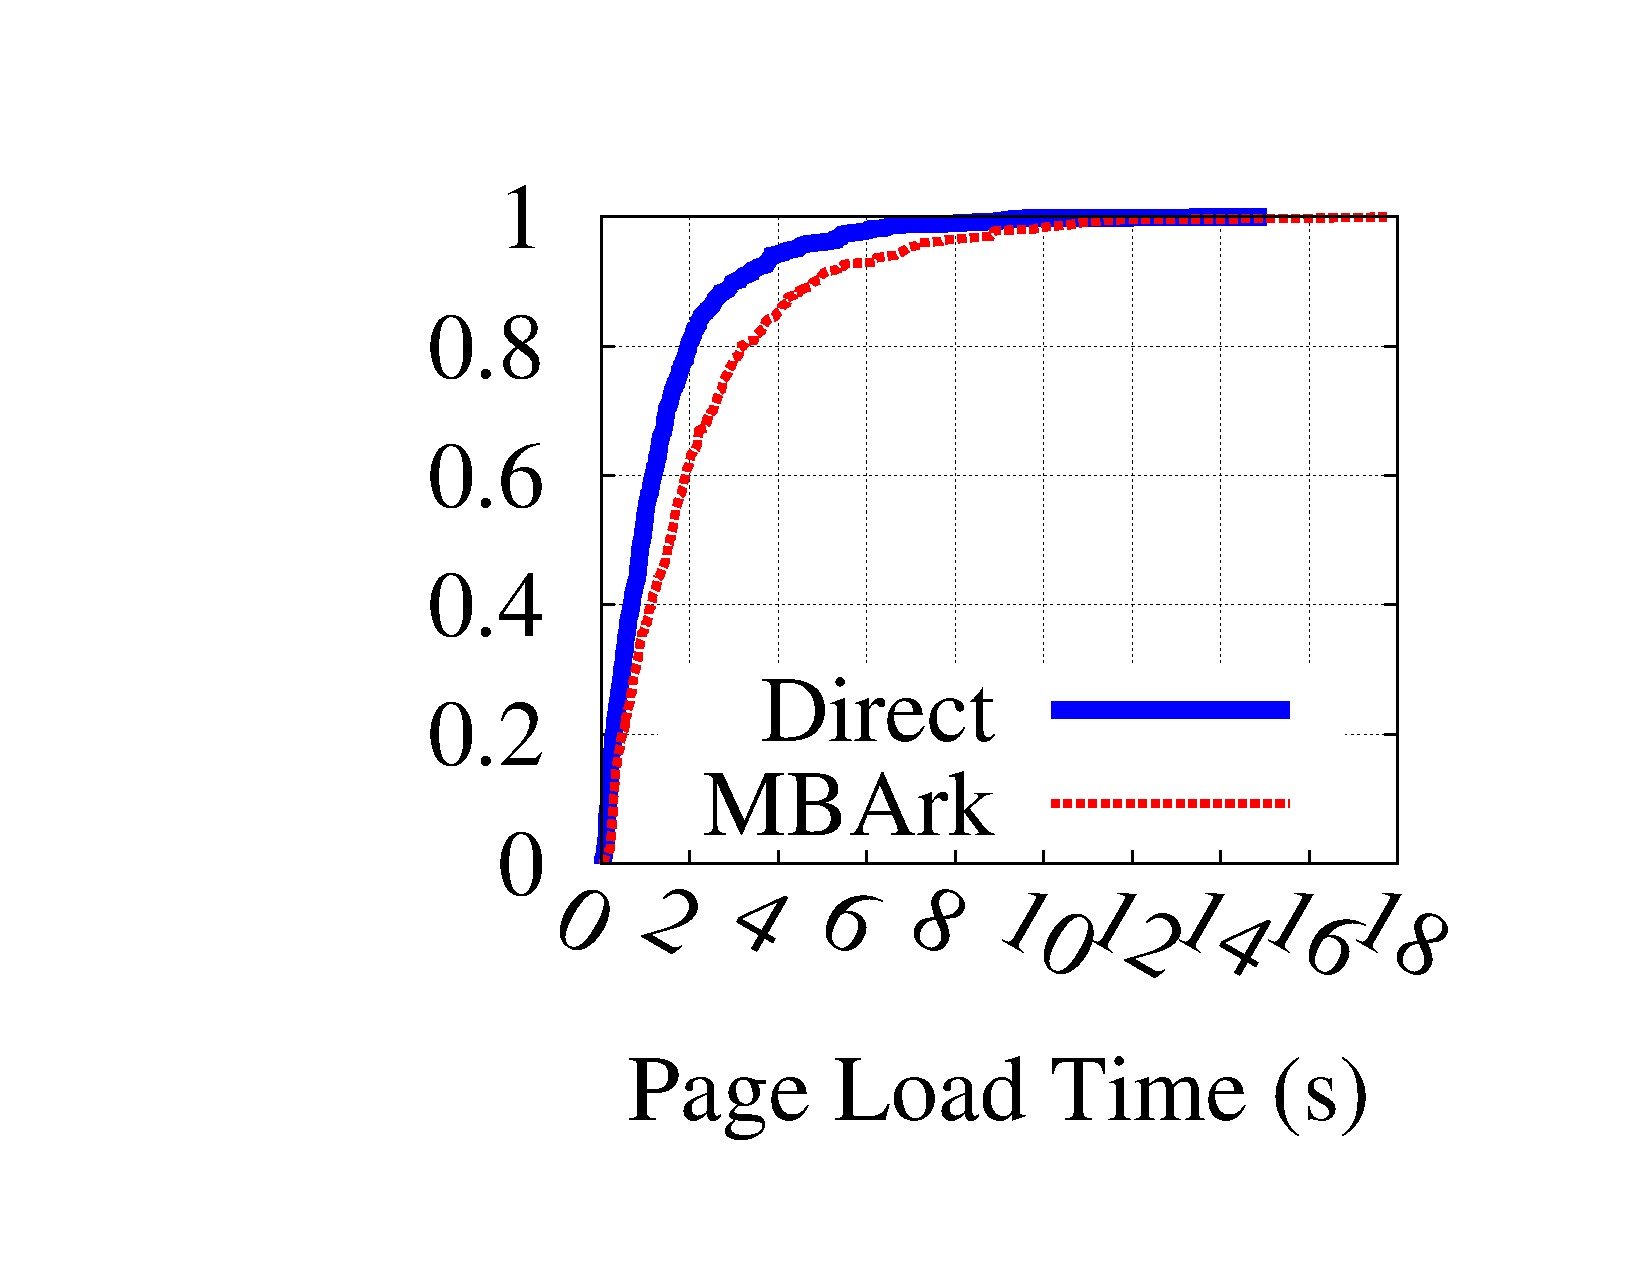
\includegraphics[height=.9in]{fig/e2e_loadtimes}
%  &\hspace{-10pt}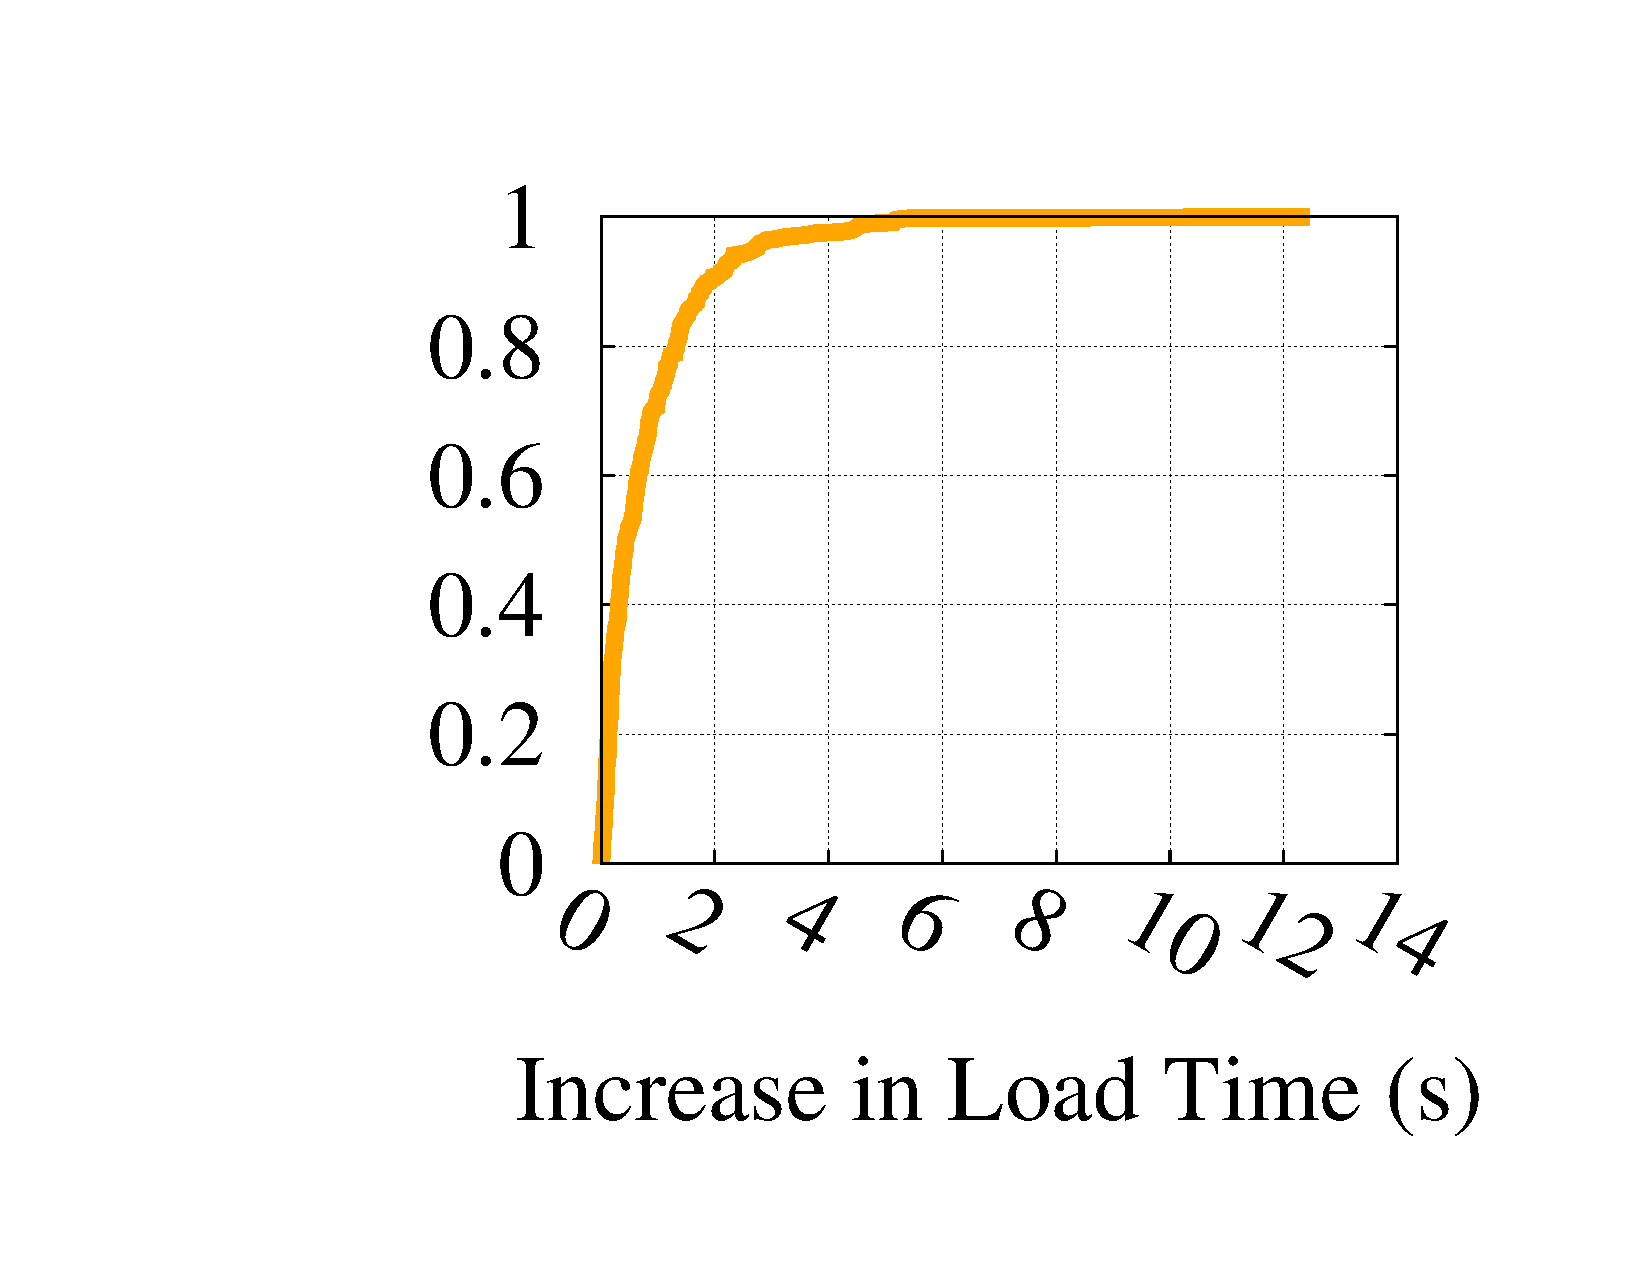
\includegraphics[height=.9in]{fig/e2e_delta_absolute}
%  &\hspace{-10pt}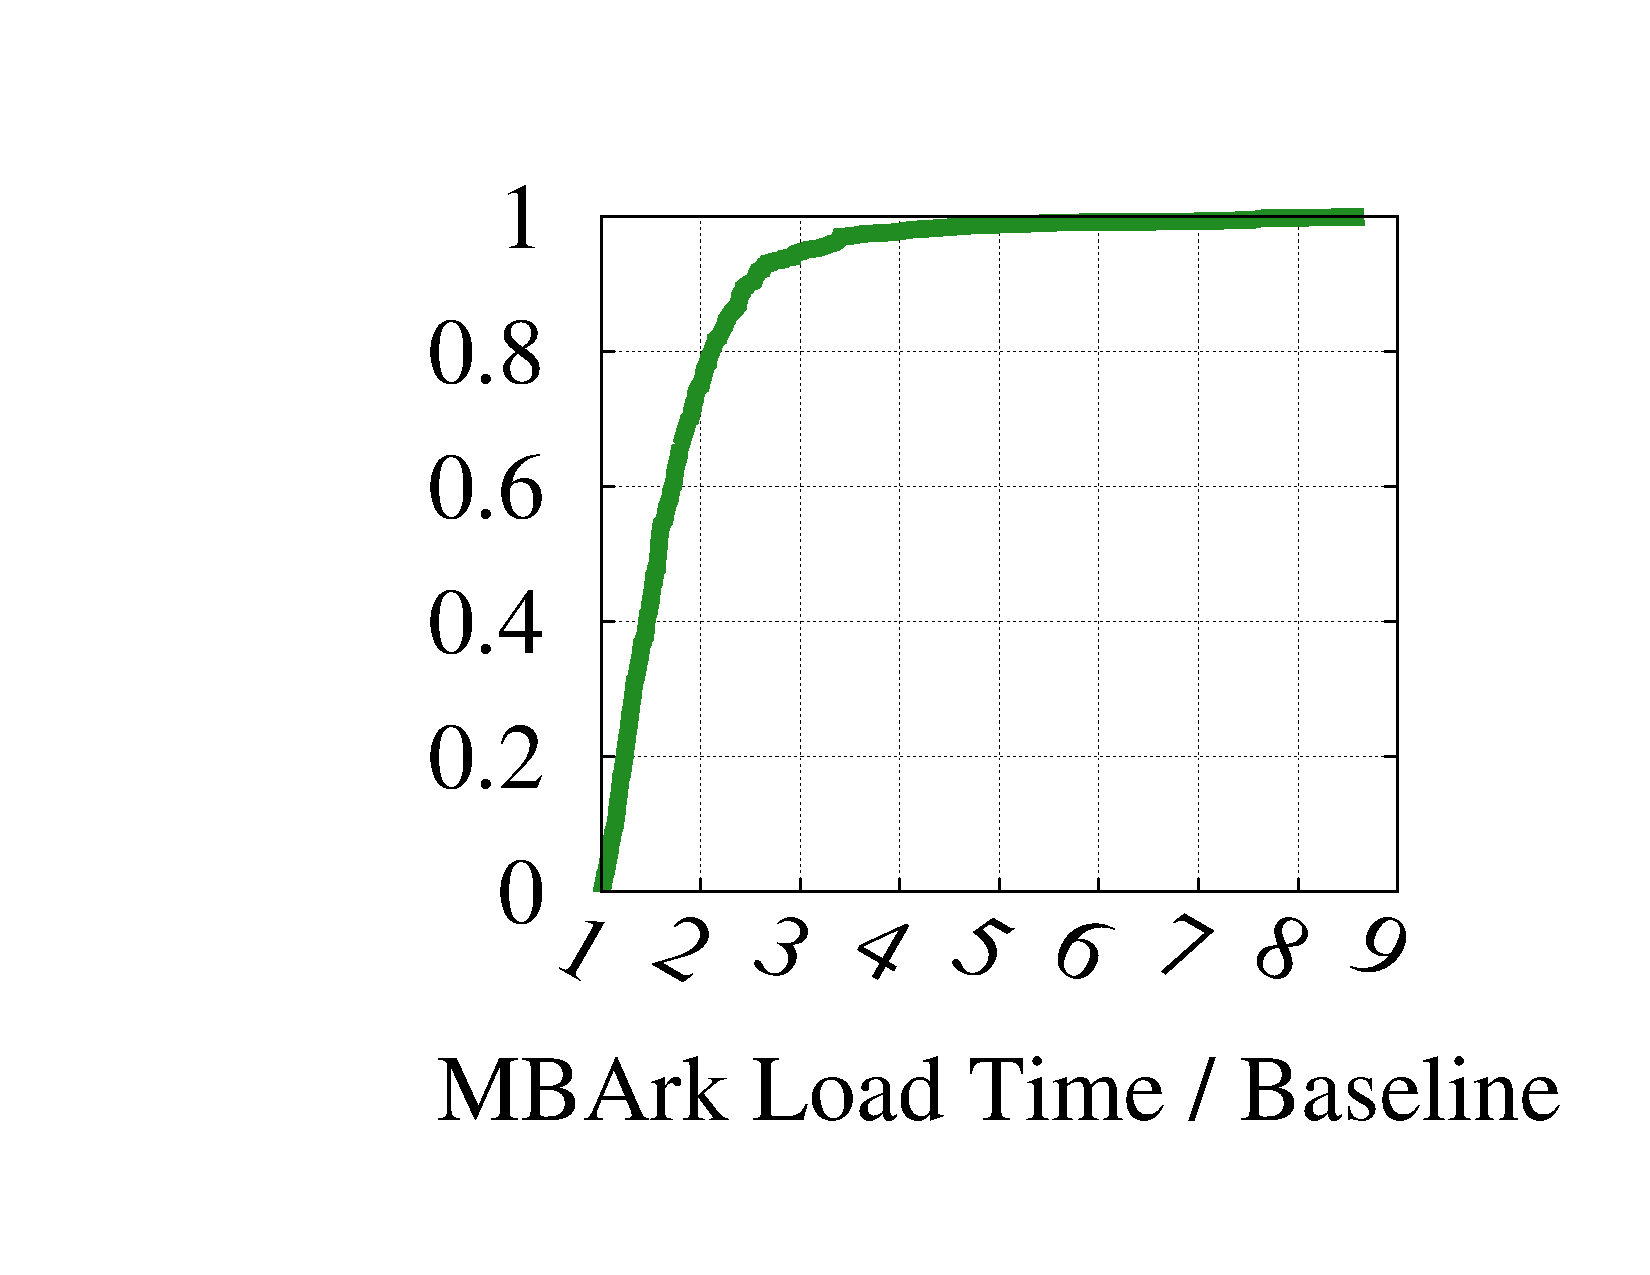
\includegraphics[height=.9in]{fig/e2e_delta_relative}
%  \\
%  &(a)&(b)&(c)\\
%  \end{tabular}
  \centering
  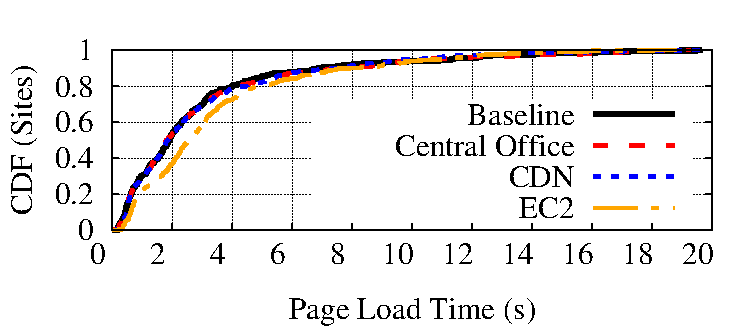
\includegraphics[width=3in]{fig/e2e_compare}
  \caption[]{\label{fig:e2eloads} Page load times under different deployments.}
\end{figure}

We use web performance to understand end-to-end client experience using \sys.
Figure~\ref{fig:e2eloads} shows a CDF for the Alexa top-500 sites loaded through our testbed. We compare the baseline (direct download) with 3 different deployment scenarios of \sys: Central Office, CDN, and Amazon EC2-like virtual private server. To measure the performance under those scenarios, we inflate the mean roundtrip latency with 60us for CO, 4ms for CDN, and 30ms for EC2. 
Because of the `bounce' redirection \sys uses, all page load times increase by only a small fraction; in the median case this increase is less than 0.05 second for CO, 0.1 second for CDN, and 0.72 second for EC2. At the 95th percentile, page loads increase by about 0.4 second for CO, 0.6 second for CDN, and 0.73 second for EC2. We conclude that the latency impact is negligible when MBArk is deployed on CO or CDN.

\subsubsection{Bandwidth Overheads}
We evaluate two costs: the increase in bandwidth due to our encryption and metadata, and the increase in bandwidth cost due to `bounce' redirection.

\noindent{\it How much does \sys encryption increase the amount of data sent to the cloud?}
The gateway inflates the size of traffic due to three encryption costs:
\begin{CompactItemize}
  \item If the enterprise uses IPv4, there is a 20-byte per-packet cost to convert from IPv4 to IPv6. If the enterprise uses IPv6 by default, there is no such cost.
  \item If HTTP proxying is enabled, there are on average 132 bytes per request in additional encrypted data.
  \item If HTTP IDS is enabled, there is at worst a 5$\times$ overhead on all HTTP payloads.
\end{CompactItemize}
We used the m57 trace to understand how these overheads would play out in aggregate for an enterprise.
On the uplink, from the gateway to the middlebox service provider, traffic would increase by 2.5\% due to encryption costs for a Header-Only Gateway. Traffic would increase by 4.3$\times$ on the uplink for a bytestream-aware gateway. 


\noindent{\it How much does bandwidth increase between the gateway and the cloud from using \sys? How much would this bandwidth increase an enterprises networking costs?}
\sys sends all network traffic to and from the middlebox service provider for processing, before sending that traffic out to the Internet at large. In NFV contexts, the clients' middlebox service provider and network connectivity provider are one and the same and one might expect costs for relaying the traffic to and from the middleboxes to be rolled in to one `package.' 
However, in the APLOMB setting, the middlebox service provider is a cloud, meaning that the client must pay a third party ISP to transfer the data to and from the cloud, before paying that ISP a third time actually transfer the data over the network.

Using current bandwidth pricing~\cite{comcast-costs, megapath-costs, verizon-costs}, we can estimate how much outsourcing would increase overall bandwidth costs.
Multi-site enterprises typically provision two kinds of networking costs: Internet access, and intra-domain connectivity. 
Internet access typically has high bandwidth but a lower SLA -- 99 or 99.5\% uptime; traffic may also be sent over shared Ethernet~\cite{comcast-costs, verizon-costs}.
Intra-domain connectivity usually has a private, virtual Ethernet link between sites of the company with a high SLA (over 99\%) and lower bandwidth.
This latter connectivity tends to cost about two orders of magnitude more than the former, because of the high SLA, extra configuration, and support required.
Because bounce redirection is over the `cheaper' link, the overall impact to bandwidth cost with header-only encryption given public sales numbers is between 15-50\%; with bytestream aware encryption this cost increases to between 30-150\%. 

\eat{Getting frustrated with these numbers so leaving them here and will come back to them. Megapath offers a dedicated link at 5x5Mbps for \$250/mo; 20x20Mbps for \$1300/mo. Comcast offers enterprise cable at 150/20Mbps for \$250/mo. The three way bounce should result in a cost increase of 15-50\%, depending on how much the internal link is providioned for. The DPI should be 2-3 times that, so, between 30-150\%... 
}

\subsection{Middleboxes}
\label{sec:evalcloud}

We now evaluate the performance overhead at each middlebox. Overall, we find that throughput is negligibly impacted due to \sys because \sys keeps most dataplane operations unchanged.

\begin{table}[t!]
\small
\begin{tabular}{p{2.5cm}|p{2cm}|p{2cm}}
{\bf Application} &  {\bf Baseline Throughput} & {\bf \sys Throughput} \\
\hline \hline
IP Firewall &  9.8Gbps &  9.8Gbps \\
%Application Firewall  & & \\
NAT & 3.6Gbps   &   3.5 Gbps \\
%IP Forwarding  & & \\
%VPN Gateway &  &  &  \\ 
Load Balancer L4  &9.8 Gbps & 9.8Gbps \\
%Load Balancer L7 & & & \\
%WAN optimizer  & & & \\
Web Proxy &1.1Gbps &1.1Gbps\\
%IDS & & & \\
IDS & 85Mbps & 166Mbps~\cite{blindbox}   \\
\end{tabular}
\caption{Middlebox applications supported by Header-Only \sys; throughput measured with an empirical traffic workload. \label{tbl:appsxput}}
\
\end{table}

\noindent{\it Is throughput reduced at the middleboxes due to  \sys?}
Table~\ref{tbl:appsxput} shows the throughput sustained for the apps we implemented.
The IP Firewall, NAT, and Load Balancer are all `header only' middleboxes; the results shown compare packet processing over the same dataplane, once with encrypted IPv6 data and once with unencrypted IPv4 data.
The only middlebox for which any overhead is observable is the NAT -- and this is a reduction of only 2.7\%.

We re-implemented the Web Proxy and IDS to enable the bytestream aware operations they require over our encrypted data. The Web Proxy sustains the same throughput with and without encrypted data, but, as we will present leter, does have a higher service time per cache hit.
The IDS numbers compare Snort (baseline) to the BlindBox implementation; this is not an apples-to-apples comparison as BlindBox performs mostly exact matches where Snort performs regular expressions.

In what follows, we provide some further middlebox-specific benchmarks for the firewall, proxy, and IDS.

\noindent{\bf Firewalls:} 
{\it Does \sys support all rules in a typical firewall configuration? How much does the ruleset ``expand'' due to encryption?}
We tested our firewall with three actively-used rulesets provided to us by a network administrator at our institution; two rulesets were in a proprietary firewall format and one was a set of IPTables rules for a software Linux firewall.
We were able to encode all rules using range and keyword match encryptions.

We also investigated how much the ruleset increased due to range encryption. Rules are typically encoded in the firewall as prefixes, hence a rule over the range [4.0.0.0, 4.255.255.255] is in practice implemented as a bitmask over the first 8 bits of every packet; checking to see if the packet matches the prefix 4.0.0.0/8.
Using range encryption, the same prefix might be mapped to 9.128.0.0-10.128.0.0.0, resulting in two /9 prefix ranges in the final rule encoding: 9.128.0.0/9 or 10.128.0.0/9.
As throughput for many middleboxes decreases with the number of rules, we were concerned that these mappings might degrade performance. However, in practice rules increased modestly, by between 5.8\% and 10.2\%.

\begin{figure}[t]
\centering
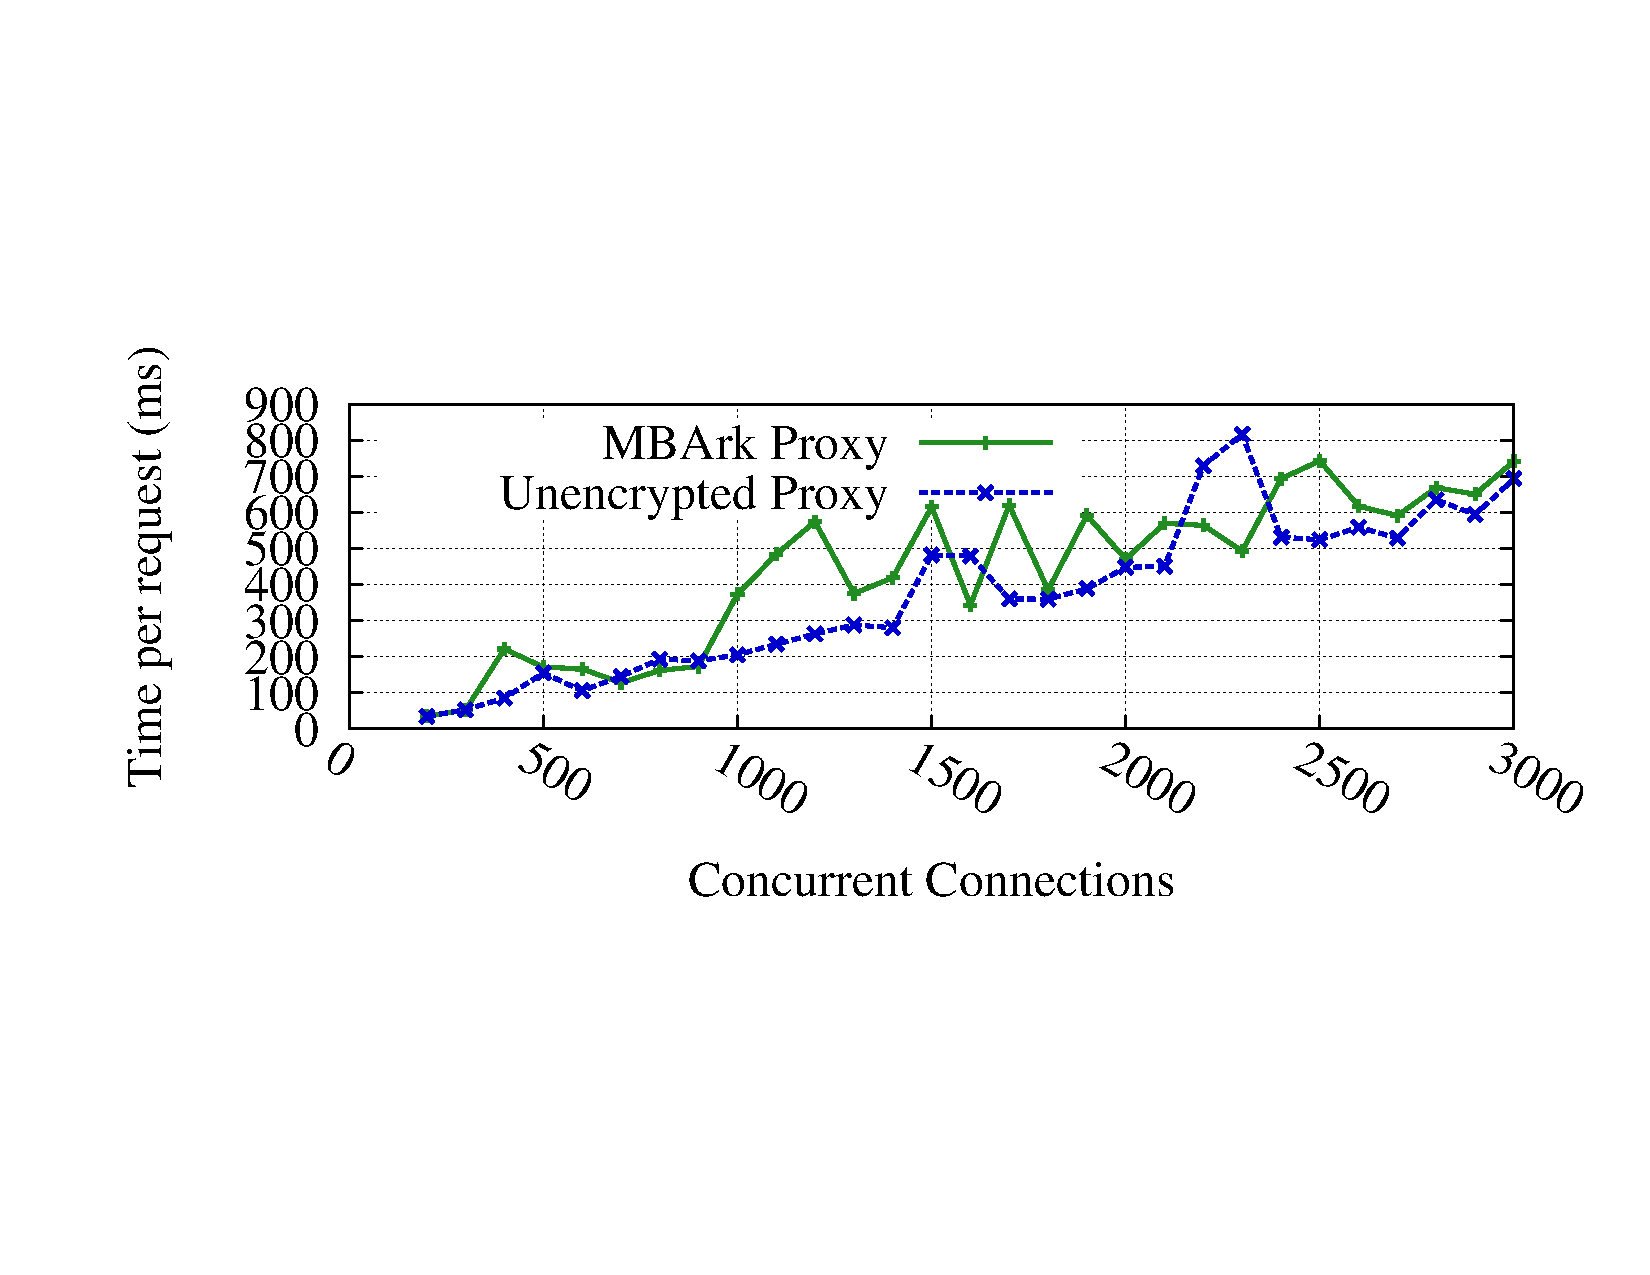
\includegraphics[width=3in]{fig/proxytime}
\caption{\label{fig:proxygraph} Access time per page against the number of concurrent connections at the proxy.}
\end{figure}

\noindent{\bf Proxy/Caching:} The throughput number shown in Table~\ref{tbl:appsxput} is not the typical metric used to measure proxy performance. A better metric for proxies is how many connections the proxy can handle concurrently, and what time-to-service it offers each client. In Figure~\ref{fig:proxygraph}, we plot time-to-service against the number of concurrent connections, and see that it is on average higher for \sys than the unencrypted proxy, by tens to hundreds of milliseconds per page.
This is not due to computation costs, but instead, due to the fact that the encrypted HTTP header values are transmitted on a different channel than the primary data connection.
The \sys proxy needs to synchronize between these two flows, reading in HTTP header values from the metadata channel and then determining which connection they belong to; this synchronization cost is what increases the time to service. The synchronization cost would go down if all of the encrypted header values were stored in the HTTP packets themselves.


\noindent{\bf Intrusion Detection:}
Our IDS is based on BlindBox~\cite{blindbox}. BlindBox incurs a substantial `setup cost' every time a client initiates a new connection. With \sys, however, the gateway and the cloud maintain one, long-term persistent connection. 
Hence, this setup cost is paid once when the gateway is initially configured. \sys also heurstically expands regular expressions in the rulesets into exact match strings. This results in two benefits:

\noindent{\it (1) End-to-end performance improves.} Where BlindBox incurs an initial handshake of 414s~\cite{blindbox} to open a new connection, clients under \sys never pay this cost; instead they perform a normal TCP or SSL handshake of only 3-5 RTTs. In our testbed, this amounts to between 30 and 100 ms, depending on the site and protocol -- an improvement of 4 orders of magnitude.

\noindent{\it (2) Security improves.} 
Using IDS rulesets from Snort, we converted regular expressions to exact match strings by building DFAs from regular expressions and heurstically expanding DFAs as many as possible into match tokens within storage constraints. With 10G memory, we were able to convert about half of all regular expressions to a finite number of exact match strings. 
Consequently, \sys can detect more then 80-88\% of attacks using the higher security level, rather than 42-67\% as with BlindBox:

\begin{table}[h]
  \centering
  \small
  \begin{tabular}{l|c|c}
  %\begin{tabular}{p{1.75in}|p{.4in}|p{.4in}}
    {{\bf Rule Set}}&{\bf Exact Match}&{\bf Prob. Cause}\\
    \hline
    \hline
    BB: Community&67\%&100\%\\
    \hline
    MB: Community&88.7\%&100\%\\

    \hline
    \hline
    BB: Emerging Threats&42\%&100\%\\
    \hline
    MB: Emerging Threats&79.8\%&100\%\\
    \hline
  \end{tabular}
\end{table}


